\section{Mapeamento e Localização}
\label{sec:mapeamento_localizacao}

%A questão do mapeamento e localização é considerado um problema central na
%robótica móvel, 

O mapeamento e localização é uma necessidade recorrente nas aplicações em
robótica móvel, onde a caracterização do veículo como autônomo de fato pode vir
a ser dada essencialmente pela sua capacidade de tratar esta questão. Para que
um robô possa ir de um ponto ao outro do ambiente ele deve conhecer, pelo menos,
a sua localização e a localização do seu ponto de destino. Quando o mapa e a
estrutura do ambiente, assim como a localização do veículo, são desconhecidos a
priori essa questão se torna crítica. Esta necessidade é denominado de SLAM
(\textit{Simultaneous Localization and Mapping}) e é um problema central na
robótica móvel, onde ambas informações dependem uma da outra para serem obtidas. Um
algoritmo proposto para solucionar o SLAM é apresentado em \cite{Thrun2004} que
utiliza uma abordagem probabilística onde as estimativas tando da posição como
do mapeamento são atualizadas uma a partir da outra a medida que dados
sensoriais são coletados.

A visão computacional tem sido aplicada em soluções para o tratamento de SLAM
como a fonte de informação sensorial. Outros equipamentos, como sensor a laser
utilizado em \\\cite{Lategahn2011} e até mesmo sensores inerciais (IMU -
\textit{Inertial Measurement Unit}), como apresentado em \cite{FootSLAM}, são
aplicados e combinados com o propósito de aumentar a acurácia destas medições.
% a localização é estimada pelo onde o erro da estimativa da localização reduz a
% medida que o mapeamento Esse problema é normalmente tratado através de
% abordagens como o SLAM (\textit{Simultaneous Location and Mapping}).
% Uma solução robusta e eficiente para a questão de localização e mapeamento
% simultâneos (SLAM) na prática ainda é desafiadora (\cite{Dissanayake2001}) A
% visão computacional tem sido aplicada em soluções para o tratamento de SLAM ,
% onde uma abordagem recorrente no tratamento da localização e do mapeamento é a
% utilização de visão computacional.
% Porém há uma diversidade de sensores que podem ser integrados com o propósito
% de aumentar a acurácia destas medições, trabalhos recentes como o de
% \cite{FootSLAM} apresenta uma abordagem baseada em sensores inerciais (IMU -
% \textit{Inertial Measurement Unit}).
Entretanto, em ambientes externos (\textit{outdoor}) e extensos a construção de
um mapa global a partir dos dados sensoriais pode não ser viável, comprometendo
a estimação da localização baseada em mapa.
% e a definição da localização em relação a este mapa pode se tornar um problema
% intratável .
Uma solução para determinação da localização em ambientes externos é a obtenção
de coordenadas através do uso do GPS (\textit{Global Positioning System}), que é
baseado na trilateração das distâncias do veículo em relação a uma “constelação”
de satélites deste sistema. Portanto, a posição do veículo e de seu destino pode
ser estimada diretamente (com um certo erro) a partir das informações fornecidas
por um aparelho localizador GPS.



%OSORIO
%> Podia discutir um pouco mais sobre estas questões (expandir esta seção):
%- Dependência da existência de um mapa previamente definido (mapeado pelo robô
%ou não) e do planejamento prévio da rota do robô, ou, navegar no ambiente
%(usualmente não estruturado) sem o uso de um mapa ou de um planejamento prévio
%de rotas (existe o risco de ficar bloqueado, pois possui apenas o conhecimento
%local do ambiente e não realiza um plano global => é bom mostrar que está
%consciente disto).
%- Dependência de um mapa (global) exato e de uma localização exata, ou
%alternativamente, usa um mapa aproximado (local) e usa uma localização também
%aproximada (não muito precisa).
%> São abordagens possíveis e podemos "escolher" entre elas de acordo com o
%problema e requisitos impostos pela aplicação. Obviamente neste trabalho foi
%feita uma escolha (e espero que o leitor se convença que foi uma boa escolha
%dado o contexto)    :)


A localização pode se beneficiar quando há mapas previamente fornecidos, sendo
necessária a localização da posição inicial em relação ao mapa. Os mapas têm
papel importante na tarefa de navegação (seção \ref{sec:navegacao}), tanto
quando fornecidos previamente como quando construídos no momento em que o
veículo se desloca no ambiente. O mapa para navegação geralmente se caracteriza como
local ou global \cite{concepts}. O mapa global provê informações mais
abrangentes sobre o espaço onde o veículo irá se deslocar, principalmente
fornecendo informações sobre obstáculos estáticos e zonas navegáveis
preferenciais, como estradas. Estas informações dos mapas normalmente se
associam a custos, os quais são utilizados pelos algoritmos de planejamento
buscar o melhor caminho. Também, os mapas podem ser representados de forma
métrica (geométrica) e/ou topológica - contendo informações mais detalhadas de o
quê ocupa um determinado espaço (prédio, vegetação, etc.)\cite{Thrun98a}. Já os
mapas locais têm o papel de expressar o ambiente dentro do raio de atuação dos
sensores, ou seja, uma noção localizada próxima ao veículo. Estes mapa local
contém a visão mais atual do ambiente, contemplando obstáculos dinâmicos. A
construção do mapa local pode ser utilizado para agregar informações e atualizar
o mapa global, desta forma, o mapa global se traduz em uma memória do espaço
para o veículo (\fig{fig:map2d}). Quando não há informação prévia que possa ser
utilizada como mapa global é usual uma navegação prévia para o reconhecimento do
ambiente antes que se efetuem tarefas específicas de navegação. Este
reconhecimento inicial pode ser feito de forma autônoma apenas vagando no
ambiente como uma navegação guiada.

\begin{figure}[ht]
%	\centering
	\begin{minipage}[b]{0.9\linewidth}
	    \centering
	    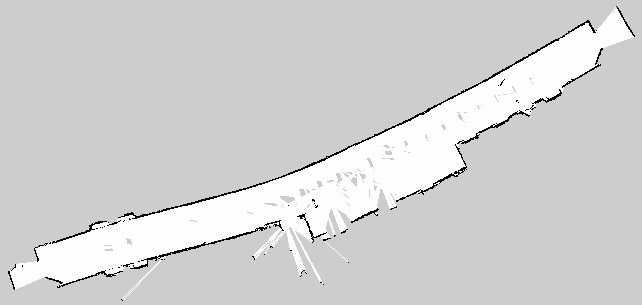
\includegraphics[width=\textwidth,height=6cm]{images/map_2d.jpg}
	 	\caption{Mapa de ocupação planar: Em branco o espaço live, em preto o espaço
	 	ocupado e em cinza o espaço sem informação de ocupação}
		\fonte{www.ros.org (divulgação)}
	 	\label{fig:map2d}
	\end{minipage}
\end{figure}

%2012-10-15 Lido OK (pode ainda ser mais desenvolvido)

